% !TEX TS-program = xelatex
% !TEX encoding = UTF-8 Unicode

\documentclass[11pt,tikz,border=1]{standalone}
\usepackage[default,mdseries=Light,bfseries=Medium,path=fonts]{cjkfonts}
\usetikzlibrary{calc,positioning,arrows.meta,shapes.geometric,shapes.misc}
\usepackage{pgfplots}

\begin{document}
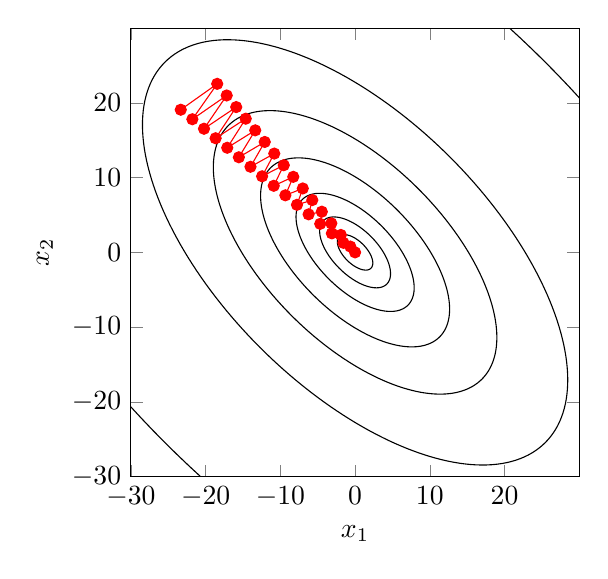
\begin{tikzpicture}
  
    \begin{axis}[
      xlabel={$x_1$},
      % x label style={yshift=0.5em},
      ylabel={$x_2$},
      % y label style={yshift=-1em},
      xtick={-30, -20, -10, 0, 10, 20},
      ytick={-30, -20, -10, 0, 10, 20},
      xmin=-30,
      xmax=30,
      ymin=-30,
      ymax=30,
      unit vector ratio*=1 1 1]

    \addplot[
      domain=0:2*pi,
      samples=201,
      rotate around={-45:(axis cs:0,0)}
    ](
      {72 * cos(deg(x))},
      {36 * sin(deg(x))}
    );
    
    \addplot[
      domain=0:2*pi,
      samples=201,
      rotate around={-45:(axis cs:0,0)}
    ](
      {36 * cos(deg(x))},
      {18 * sin(deg(x))}
    );

    \addplot[
      domain=0:2*pi,
      samples=201,
      rotate around={-45:(axis cs:0,0)}
    ](
      {24 * cos(deg(x))},
      {12 * sin(deg(x))}
    );

    \addplot[
      domain=0:2*pi,
      samples=201,
      rotate around={-45:(axis cs:0,0)}
    ](
      {16 * cos(deg(x))},
      {8 * sin(deg(x))}
    );

    \addplot[
      domain=0:2*pi,
      samples=201,
      rotate around={-45:(axis cs:0,0)}
    ](
      {10 * cos(deg(x))},
      {5 * sin(deg(x))}
    );

    \addplot[
      domain=0:2*pi,
      samples=201,
      rotate around={-45:(axis cs:0,0)}
    ](
      {6 * cos(deg(x))},
      {3 * sin(deg(x))}
    );

    \addplot[
      domain=0:2*pi,
      samples=201,
      rotate around={-45:(axis cs:0,0)}
    ](
      {3 * cos(deg(x))},
      {1.5 * sin(deg(x))}
    );
    
    % FIXME: just looks the similar, not accurate
    \addplot[
      red,
      mark=*,
      rotate around={135:(axis cs:0,0)}
    ] coordinates {
      (0, 0)
      (1, -0.1)
      (2, 0.2)
      (3, -0.3)
      (4, 0.4)
      (5, -0.5)
      (6, 0.6)
      (7, -0.7)
      (8, 0.8)
      (9, -0.9)
      (10, 1.0)
      (11, -1.1)
      (12, 1.2)
      (13, -1.3)
      (14, 1.4)
      (15, -1.5)
      (16, 1.6)
      (17, -1.7)
      (18, 1.8)
      (19, -1.9)
      (20, 2.0)
      (21, -2.1)
      (22, 2.2)
      (23, -2.3)
      (24, 2.4)
      (25, -2.5)
      (26, 2.6)
      (27, -2.7)
      (28, 2.8)
      (29, -2.9)
      (30, 3.0)
    };
       
%    \coordinate (o) at (axis cs:0,0);
%    \coordinate (a) at (axis cs:{cos(45)},{sin(45)});
%    \coordinate (b) at (axis cs:{cos(45)},{sin(-45)});
%    \coordinate (c) at (axis cs:{3*cos(45)},{3*sin(45)});
%    \coordinate (d) at (axis cs:{0.5*cos(45)},{0.5*sin(-45)});
%    
%    \draw[-{Latex[]}] (o) to (a);
%    \draw[-{Latex[]}] (o) to (b);
%    \draw[-{Latex[]}] (o) to (c);
%    \draw[-{Latex[]}] (o) to (d);
%    
%    \node[anchor=south west,xshift=-1mm,yshift=-3mm] at (a) {\footnotesize$v^{(1)}$};
%    \node[anchor=west,xshift=-1mm,yshift=2mm] at (b) {\footnotesize$v^{(2)}$};
%    \node[anchor=south west,xshift=-2mm,yshift=-1mm] at (c) {\footnotesize$\lambda_1v^{(1)}$};
%    \node[anchor=west,xshift=-1mm,yshift=2mm] at (d) {\footnotesize$\lambda_2v^{(2)}$};
    
  \end{axis}
  
\end{tikzpicture}
\end{document}
